\chapter{Real-Time MRI: State of the Art} \label{Chp:rtMRI}
\chaptermark{Real-Time MRI}

Real-time MRI refers to high-speed MRI acquisitions at millisecond resolution. Initially, spiral sampling was proposed for real-time cardiac MRI \cite{2004_rt_spiral} and further developed in HeartVista\texttrademark\footnote{\url{https://www.heartvista.com/}}. For accelerated MRI acquisitions, spiral sampling usually has long readouts, which are prone to off-resonance-induced image artifacts (e.g.~see \cref{Sec:mri-ktrj}). Therefore, this chapter focuses on the real-time \acs{MRI} technique developed in Biomedizinische NMR Forschungs GmbH\footnote{\url{http://www.biomednmr.mpg.de/}}. Essentially, this technique comprises highly undersampled radial \acs{FLASH} acquisitions without any physiological triggering and the nonlinear inverse image reconstruction that accurately estimates both the object image and the coil sensitivity maps. 


\section{Undersampled Radial FLASH} \label{Sec:rtmri-rfl}
Radial sampling has regained great interest in the last decade. First, it is less sensitive to motion-induced ghost artifacts as commonly seen in Cartesian sampling, because the center of k-space is measured by every spoke. However, rapid motions may cause streaking artifacts in radial sampling. Second, radial sampling is resistant to spatial distortion in case of undersampling. Undersampling induces radial streaks as well, which, however, has been proven incoherent and hence can be better suppressed than coherent artifacts (e.g.~the aliasing or fold-in artifact in Cartesian undersampling). Third, as radial sampling contains two readout gradients (see \cref{Equ:mri_grad_rad}) rather than one readout and one phase-encoding gradient, it is feasible to employ oversampling along the readout directions, which effectively enlarges the circular-supported \acs{FOV} and hence reduces aliasing artifacts without additional measuring times. Due to these favorable properties, undersampled radial FLASH was proposed by Zhang et al.~in 2010 \cite{2010_rfl_JMRI} for real-time MRI.

\begin{figure}[tb]
  \centering
  \includegraphics[width = 1.0\textwidth]{fig/rtmri-seq-rad.png}
  \caption{Undersampled radial FLASH sequences. (a) RF-spoiled radial FLASH for $T_1$-weighted imaging. (b) Refocused radial FLASH for $T_1$/$T_2$-weighted imaging. (c) Undersampled radial sampling (3 spokes per frame) with 5 sequential turns.} \label{Fig:rtmri-seq-rad}
\end{figure}
Based on radial sampling, three types of sequences have been implemented for real-time MRI: spoiled and refocused radial FLASH, and balanced steady-state free precession (\acs{bSSFP}). Beside the standard \acs{RF}-spoiling, spoiled radial FLASH (see \cref{Fig:rtmri-seq-rad}a) requires no additional rewinder gradients on the readout axes as their gradient areas vary from \acs{TR} to TR interval. The resulting image contrast in spoiled radial FLASH with short \acs{TE} and TR and low flip angle (e.g.~\ang{8}) is $T_1$-weighted. This sequence has been applied primarily to phase-contrast flow velocity quantification, real-time speech imaging, and cardiovascular magnetic resonance (\acs{CMR}) imaging. On the contrary, refocused radial FLASH (see \cref{Fig:rtmri-seq-rad}b) renders $T_2$/$T_1$-weighted image contrast and hence has been intensively used for the diagnosis of temporomandibular joint (TMJ) dysfunctions. To achieve steady state, furthermore, refocused radial FLASH does not spoil the transverse magnetization, but requires it to be consistent among TR intervals, and thus rewinder gradient is employed on both the two readout gradients. Another conventional and appealing CMR imaging sequence is \acs{bSSFP}, which offers $T_2$/$T_1$-weighted image contrast as well. bSSFP requires zero gradient area on all gradient axes, so it has an additional rewinder gradient on the slice selection gradient when compared to refocused radial FLASH. Nevertheless, bSSFP provides excellent contrast between myocardium (heart muscle) and flowing blood as myocardium has a lower $T_2$/$T_1$ ratio compared to blood. The application of bSSFP to real-time CMR imaging at \SI{1.5}{\tesla} with an achievable temporal resolution of \SI{40}{\ms} has been developed by Voit et al.~in 2013 \cite{2013_SSFP_Voit}. One drawback of bSSFP, however, is that it is prone to banding artifacts due to the off-resonance phase modulation. 

As shown in \cref{Fig:rtmri-seq-rad}c, one image frame (\textit{turn}) comprises a certain number of spokes (e.g.~$N_S = 3$), which are uniformly distributed in k-space and sequentially rotated between successive turns. Moreover, the radial sampling pattern is repeated every $N_T$ turns (e.g.~$N_T = 5$). In the current implementation of real-time MRI sequences, both $N_S$ and $N_T$ are limited to odd integers as a consequence of the total radial angle coverage set to be $2\pi$. The angle increment between two successive spokes ($\Delta \theta_{\text{spoke}}$) and that between two successive turns ($\Delta \theta_{\text{turn}}$) can be given as 
\begin{align}
  \Delta \theta_{\text{spoke}} &= 2\pi / N_S \\
\intertext{and}
  \Delta \theta_{\text{turn}}  &= 2\pi / (N_S \cdot N_T) \quad ,\\
\intertext{respectively. Therefore, the angle of the $s^{\text{th}}$ spoke in the $m^{\text{th}}$ frame is}
  \theta (s, m) &= [ (m-1) \mod{N_T} ] \cdot \Delta \theta_{\text{turn}} + (s-1) \cdot \Delta \theta_{\text{spoke}} \quad . \label{Equ:rtmri-spk-ang}
\end{align}

\section{Parallel Imaging as Nonlinear Inverse Problem} \label{Sec:rtmri-nlinv}
Prior to the nonlinear inversion (\acs{NLINV}) reconstruction for parallel imaging \cite{2007_IRGNM_PI,2008_NLINV,2010_NLINV_Heart,2010_20ms_Uecker}, joint sensitivity encoding (\acs{JSENSE}) \cite{2007_JSENSE} had been proposed by Ying et al.~in 2007 to ``jointly" estimate image content and coil sensitivity maps. However, JSENSE updates the estimate image and coil sensitivity maps in an alternative manner -- the image is estimated via CG-SENSE with the current estimate coil sensitivity maps fixed, and then coil sensitivity maps are estimated via the CG-type method with the current estimate image fixed. In short, this method separates a nonlinear inverse problem into two linear inverse problems and solve them alternatively. NLINV is the first algorithm that jointly estimates image content and coil sensitivity maps via the iteratively regularized Gauss-Newton method (\acs{IRGNM}) \cite{1996_regu_inv,2004_iter_inv}. 

\subsection*{Algorithm}
Following \cref{Equ:mri-pi-forward}, the system equation in parallel imaging can be written as
\begin{equation} \label{Equ:rtmri-nlinv-system}
  y = F(x) \quad \text{with} \; x = 
  \left( \begin{array} {c}
    \rho \\
    c_1 \\
    \vdots \\
    c_N \\
  \end{array} \right)
\end{equation}
with both the image ($\rho$) and coil sensitivity maps being the unknown ($x$). Here, it is convenient to denote the forward operation on the $n$\textsuperscript{th} coil as $F_n (x) = P \mathcal{F} \{ \rho \cdot c_n \}$.

\cref{Equ:rtmri-nlinv-system} represents a \textit{nonlinear} system because when assuming $x_1 = (\rho_1,~c_1)^T$ and $x_2 = (\rho_2,~c_2)^T$, a linear system satisfies $F(x_1) + F(x_2) = F(x_1 + x_2)$, but 
\begin{align*}
  F(x_1) + F(x_2) 
  &= P \mathcal{F} \{ \rho_1 \cdot c_1 \} + P \mathcal{F} \{ \rho_2 \cdot c_2 \} \\
  &= P \mathcal{F} \{ \rho_1 \cdot c_1 + \rho_2 \cdot c_2 \} \quad , \\
\intertext{which is not equal to} 
  F(x_1 + x_2) 
  &= F \begin{pmatrix}
    \rho_1 + \rho_2 \\
    c_1 + c_2
  \end{pmatrix} \\
  &= P \mathcal{F} \{ (\rho_1 + \rho_2) \cdot (c_1 + c_2) \} \quad .
\end{align*} 
To solve this nonlinear problem, IRGNM firstly linearizes it as $y = DF(x_n) \text{d}x + F(x_n)$, where $x_n$ is the estimate from $n^{\text{th}}$ Newton step and $DF(x_n)$ is the Frech\'et derivative. Thus, the cost function in \cref{Equ:mri_inv_cost} becomes 
\begin{equation} \label{Equ:rtmri-nlinv-cost}
  \Phi(\text{d}x) = \argmin\limits_{\text{d}x} \norm{DF(x_n)\text{d}x - [y - F(x_n)]}_2^2 + \alpha_n \norm{W ( x_n + \text{d}x - x_0 )}_2^2
\end{equation}
with $\alpha_n$ being the Tikhonov regularization parameter, $x_0$ the initial guess, which is initialized by the estimate from the preceding frame damped by a dampening factor $p$ ($0 \leq p \leq 1$). To counteract the ill-condition of this inverse problem, the unknown $x$ is subject to a transformation by the preconditioning matrix $W$, 
\begin{equation} \label{Equ:rtmri-nlinv-W}
  \hat{x} = 
  \left( \begin{array}{c}
    \rho \\
    \hat{c}_1 \\
    \vdots \\
    \hat{c}_N \\
  \end{array} \right) = 
  \begin{pmatrix}
    I &                                             &        & \\
      & \Big( 1 + s \norm{\vec{k}}_2^2 \Big)^{-l} \mathcal{F} &        & \\
      &                                             & \ddots & \\
      &                                             &        & \Big( 1 + s \norm{\vec{k}}_2^2 \Big)^{-l} \mathcal{F}
  \end{pmatrix} 
  \left( \begin{array}{c}
    \rho \\
    c_1 \\
    \vdots \\
    c_N \\
  \end{array} \right)
\end{equation}
with $\vec{k}$ being 2D Cartesian grid, $s = 440$, and $l = 16$. This transformation ensures the spatial smoothness of coil sensitivity maps, as the signal from high spatial frequency region is strongly penalized. With this preconditioning, the cost function can be solved via conjugate gradient method with Tikhonov regularization. The optimized $\text{d}x$ is then used to update $x_{n+1}$: $x_{n+1} = x_n + \text{d}x$. Beside the forward operator $F(x)$, the solution of \cref{Equ:rtmri-nlinv-cost} requires $DF(x)$ and its adjoint $DF^{H} (x)$. A fast forward computation of $DF(x)$ can be derived via the Jacobian matrix
\begin{align}
  DF(x) \begin{pmatrix}
    \text{d} \rho \\
    \text{d} c_1 \\
    \vdots \\
    \text{d} c_N
  \end{pmatrix} 
  &= \begin{pmatrix}
    \frac{\partial}{\partial \rho} F_1 (x) & \frac{\partial}{\partial c_1} F_1 (x) & \cdots & \frac{\partial}{\partial c_N} F_1 (x) \\
    \frac{\partial}{\partial \rho} F_2 (x) & \frac{\partial}{\partial c_1} F_2 (x) & \cdots & \frac{\partial}{\partial c_N} F_2 (x) \\
    \vdots & \vdots & \ddots & \vdots \\
    \frac{\partial}{\partial \rho} F_N (x) & \frac{\partial}{\partial c_1} F_N (x) & \cdots & \frac{\partial}{\partial c_N} F_N (x) 
  \end{pmatrix} \begin{pmatrix}
    \text{d} \rho \\
    \text{d} c_1 \\
    \vdots \\
    \text{d} c_N
  \end{pmatrix} \nonumber \\
  &= \begin{pmatrix}
    P\mathcal{F}c_1 & P\mathcal{F}\rho & 0                & \cdots & 0 \\
    P\mathcal{F}c_2 & 0                & P\mathcal{F}\rho & \cdots & 0 \\
    \vdots          & \vdots           & \vdots           & \ddots & \vdots \\
    P\mathcal{F}c_N & 0                & 0                & \cdots & P\mathcal{F}\rho
  \end{pmatrix} \begin{pmatrix}
    \text{d} \rho \\
    \text{d} c_1 \\
    \vdots \\
    \text{d} c_N
  \end{pmatrix} \nonumber \\
  &= \begin{pmatrix}
    P\mathcal{F} \{ c_1 \cdot \text{d}\rho + \rho \cdot \text{d} c_1 \} \\
    \vdots \\
    P\mathcal{F} \{ c_N \cdot \text{d}\rho + \rho \cdot \text{d} c_N \} 
  \end{pmatrix} \quad . \label{Equ:rtmri-nlinv-der} 
\end{align}
$DF^{H} (x)$ can then be exploited by taking the conjugate transpose of $DF(x)$
\begin{align}
  DF^{H} (x) \begin{pmatrix}
    \text{d} y_1 \\
    \vdots \\
    \text{d} y_N
  \end{pmatrix}
  &= \begin{pmatrix}
    c_1^* \mathcal{F}^{-1} P^H & c_2^* \mathcal{F}^{-1} P^H & \cdots & c_N^* \mathcal{F}^{-1} P^H \\
    \rho^* \mathcal{F}^{-1} P^H & 0 & \cdots & 0 \\
    0 & \rho^* \mathcal{F}^{-1} P^H & \cdots & 0 \\
    \vdots & \vdots & \ddots & \vdots \\
    0 & 0 & \cdots & \rho^* \mathcal{F}^{-1} P^H
  \end{pmatrix} \begin{pmatrix}
    \text{d} y_1 \\
    \vdots \\
    \text{d} y_N
  \end{pmatrix} \nonumber \\
  &= \begin{pmatrix}
    \sum_{n=1}^{N} c_n^* \cdot \mathcal{F}^{-1} P^H \text{d} y_n \\
    \rho^* \cdot \mathcal{F}^{-1} P^H \text{d} y_1 \\
    \vdots \\
    \rho^* \cdot \mathcal{F}^{-1} P^H \text{d} y_N 
  \end{pmatrix} \quad . \label{Equ:rtmri-nlinv-adj}
\end{align}
With these two operators, the update rule of $\text{d}x$ can be derived from \cref{Equ:rtmri-nlinv-cost}
\begin{equation} \label{Equ:rtmri-dx-sol}
  \text{d}x = [DF(x_n)^H DF(x_n) + \alpha_n I]^{-1} \{ DF(x_n)^H [y-F(x_n)] + \alpha_n (x_0 - x_n) \}
\end{equation}

For the reconstruction of serial images via real-time MRI acquisitions, the algorithm is initialized with $\rho=1$ and $c_n = 0$ for the first frame, while the following frames are initialized with the estimate from the preceding frame, which effectively acts as temporal regularizations. The incorporation of the temporal regularization into NLINV enforces temporal correlations among successive image frames. The regularization parameter decays along Newton steps according to $\alpha_n = \alpha_0 \cdot 2^{-n}$ and $\alpha_0 = 1$.

As the iterative NLINV image reconstruction technique is of heavy computational load and time consuming, it has been implemented on multiple graphics processing units (\acsp{GPU}) and fully integrated into the reconstruction pipeline of the MRI system \cite{2012_Schaetz}. 

\subsection*{Preprocessing}
Before NLINV image reconstructions, the acquired multi-channel k-space data is firstly corrected for gradient delays \cite{2011_GDC}, then compressed to \num{10} virtual channels via principle component analysis, and finally gridded onto 2D Cartesian grids without density compensation and normalized to \num{100} in the $L^2$ norm. On the other hand, the sampling pattern $P$ (refer to \cref{Equ:mri-pi-forward}) is the projection onto the measured k-space positions.

\subsection*{Postprocessing}
A temporal median filter with a window size equivalent to the number of turns can be applied to the reconstructed images. Furthermore, a modified version of the non-local means denoising \cite{2005_NLM} algorithm has been developed and integrated into the online reconstruction pipeline by Klosowski et al.~\cite{2016_NLM}. 


\section{Real-Time Phase-Contrast Flow MRI} \label{Sec:rtmri-pc}

\subsection{Physical Principles}
Real-time phase-contrast flow MRI has been an important technique as it provides quantitative information for the evaluation of cardiovascular diseases. Phase-contrast flow MRI is based on the discovery by Hahn in 1960 \cite{1960_PC_Hahn} which states that velocities of flowing spins can be encoded into the phase via a bipolar gradient, under which the temporal evolution of phases can be mathematically expressed as 
\begin{align} 
  \phi(t) &= \gamma \int_{0}^{T} G(t) x(t) \text{d} t \nonumber \\
          &= \gamma \int_{0}^{T} G(t) (x_0 + v_0 t + \frac{1}{2} a_0 t^2 + \cdots ) \text{d} t \quad \text{(Taylor Series)} \nonumber \\
          &= \gamma x_0 \int_{0}^{T} G(t) \text{d} t + \gamma v_0 \int_{0}^{T} G(t) t \text{d} t + \cdots \label{Equ:rtmri-pc-math}
\end{align}
the first two integrals of which represent the phase for the static spins at location $x_0$ without macroscopic movements and the flowing spins with a constant moving velocity $v_0$, respectively. According to this equation, both spins have zero phase by the end of the flow-compensation (also named velocity-compensation) gradient ($G_{\text{FC}}$) with the waveform $1 \bar{2} 1$, as depicted in the left part of \cref{Fig:rtmri-pc-theory}. With the velocity-encoding (also named flow-encoding) gradient ($G_{\text{VENC}}$) with the waveform $1 \bar{1}$, however, the static spins still result in zero phase and the flowing spins with constant velocity have a net phase, 
\begin{align} 
  \phi_v (2\tau) &= \gamma v_0 \int_{0}^{2\tau} G(t) t \text{d} t \nonumber \\
                 &= \gamma G_0 v_0 \left( \int_{0}^{\tau} t \text{d} t - \int_{\tau}^{2\tau} t \text{d} t \right) \nonumber \\
                 &= - \gamma G_0 \tau^2 v_0 \label{Equ:rtmri-pc-vel}
\end{align}
which indicates that the velocity is linearly proportional to the accumulated net phase, as depicted in right part of \cref{Fig:rtmri-pc-theory}. Therefore, the velocity-encoding (\acs{VENC}) range, determined by the velocity-encoding gradient amplitude ($G_0$) and duration ($\tau$) has to be larger than the velocity to be measured ($v$). Otherwise, the image area with exceeded velocities incurs velocity \textit{aliasing} artifacts, appearing as random phase values. However, VENC can not be arbitrarily large because the SNR of the measured phase is constrained by the VENC \cite{1991_PD_CD_PC}
\begin{equation}
  \snr_{\phi_v} \propto \snr_{\text{Mag}} \cdot \frac{\abs{v}}{\text{VENC}}
\end{equation}
with $\snr_{\text{Mag}}$ being the SNR of the measured magnitude image. Thus, imaging protocols may require several measurements until the peak velocity is free of aliasing.

\begin{figure}[tb]
  \centering
  \includegraphics[width = 1.0\textwidth]{fig/rtmri-pc-theory.png}
  \caption{Schematic illustrations of flow compensation and velocity encoding. (Left) Flow-compensation (FC) gradient with the waveform $1 \bar{2} 1$ results in zero phase for both the static spin and the spin with constant velocity. (Right) Velocity-encoding (\acs{VENC}) gradient with the waveform $1 \bar{1}$ results in zero phase for the static spin but net phase for the spin with constant velocity.} \label{Fig:rtmri-pc-theory}
\end{figure}

MR image phase, however, can have various sources, e.g.~the off-resonance-induced phase modulation. Therefore, to remove unwanted phases, at least two measurements with different velocity encodings are needed to obtain quantitative velocities. This can be implemented in two manners. The first approach is typically named two-sided velocity encoding \cite{2012_PC_SVE}, where the first measurement consists of a bipolar (e.g.~positive and negative) velocity-encoding gradient and the second one uses a velocity-encoding gradient with signs reversed. As a result, the phase difference between the two-sided measurements is $\Delta \phi = 2 \gamma G_0 \tau^2 v_0$. The second approach is named one-sided velocity encoding \cite{2012_PC_SVE}, where the first measurement employs the flow-compensation gradient to zero phases caused by motions and the second one uses the bipolar velocity-encoding gradient, and hence the phase difference between the one-sided measurements is $\Delta \phi = - \gamma G_0 \tau^2 v_0$. In principle, flow-encoding gradients can be applied in any direction to encode multi-dimensional velocities.

\subsection{Image Reconstructions}
In the current implementation of the real-time phase-contrast flow MRI sequence, only through-plane velocities are encoded via the one-sided velocity encoding, consisting of one flow-compensation and one flow-encoding acquisition. The two datasets are treated as two independent streams and separately reconstructed by NLINV except that they share the same channel compression matrix in the preprocessing process. The reconstructed image and coil sensitivity maps are combined to remove unwanted phase contributions from coils,
\begin{equation} \label{Equ:rtmri-pc-rho-coil}
  \rho_{j,l} = \frac{\rho_l \cdot c_{j,l}}{\sqrt{\sum_{j} c_{j,l} \cdot c^{*}_{j,l}}} \quad \text{with} \; j \in [1,N], \; l \in [1,2]
\end{equation}
with $j$ and $l$ being the index of coils and acquisitions respectively, and $*$ the complex conjugate. Thus, the complex phase-contrast map can be calculated via
\begin{align}
  \hat{\rho}_{\text{PC}} &= \sum_{j} \rho_{j,0} \cdot \rho^{*}_{j,1} \\
  \rho_{\text{PC}} &= \frac{\hat{\rho}_{\text{PC}}}{\sqrt{|\hat{\rho}_{\text{PC}}|}} \quad .
\end{align}

For quantitative flow evaluations, the complex phase-contrast maps are imported into CAIPI prototype software (Fraunhofer MEVIS\footnote{\url{http://www.mevis.fraunhofer.de/}}, Bremen, Germany), where two subsets of images are available, one anatomical magnitude image and one phase-difference (e.g.~velocity) map. To begin with, a region-of-interest (\acs{ROI}) in a certain magnitude image frame is manually selected, i.e., the ascending aorta lumen, which is then propagated through the entire image series. The propagation is able to capture the moving lumen. If not properly captured, manual corrections can be done afterwards. With the lumen determined from every phase-contrast map, CAIPI then calculates a list of flow parameters, e.g.~peak velocity, flow per heartbeat, flow volume, and regurgitation fraction.



